\documentclass[10pt,twocolumn]{article}

\usepackage[letterpaper,margin=0.75in]{geometry}
\usepackage{microtype}
\usepackage{amsmath}
\usepackage{amssymb}
\usepackage{booktabs}
\usepackage{graphicx}
\usepackage{tabularx}
\usepackage{caption}
\usepackage{subcaption}
\usepackage{placeins}
\usepackage{float}
\usepackage{balance}
\usepackage[numbers,sort&compress]{natbib}
\usepackage[colorlinks=true,citecolor=blue!45!black,linkcolor=blue!45!black,urlcolor=blue!45!black]{hyperref}
\usepackage{xcolor}

% Auto-generated by scripts/rebuild_all.py. Do not edit by hand.
\newcommand{\ModelCount}{9}
\newcommand{\PaperPromptCount}{989}
\newcommand{\ArcPromptCount}{195}
\newcommand{\CsqaPromptCount}{794}
\newcommand{\DerivedRowCount}{8,901}
\newcommand{\PrimaryRowCount}{8,901}
\newcommand{\MechanisticRowCount}{420}
\newcommand{\InstrumentedModelCount}{3}
\newcommand{\InstrumentedPromptCount}{3,000}
\newcommand{\MechanisticMinHeldoutRtwo}{0.76}
\newcommand{\MechanisticMaxHeldoutRtwo}{0.91}
\newcommand{\SpanEvidenceDistractorGap}{5.10}
\newcommand{\SpanMinPValue}{0.0002}
\newcommand{\SubstitutionAttentionMean}{1.18}
\newcommand{\SubstitutionMLPMean}{4.74}
\newcommand{\LateCrystallizingShare}{55\%}
\newcommand{\SwitchHeavyShare}{30\%}
\newcommand{\PooledMedianDTwo}{0.70}
\newcommand{\PooledMedianDOne}{0.89}
\newcommand{\PooledMedianDFifty}{0.94}
\newcommand{\PooledMedianDeltaTwentyOne}{0.09}
\newcommand{\PooledDeltaTwentyOneLow}{0.08}
\newcommand{\PooledDeltaTwentyOneHigh}{0.10}
\newcommand{\PooledMedianDeltaTwentyFifty}{0.15}
\newcommand{\PooledDeltaTwentyFiftyLow}{0.13}
\newcommand{\PooledDeltaTwentyFiftyHigh}{0.15}
\newcommand{\PooledDeltaTwoFiftyPct}{15\%}
\newcommand{\PooledWriteAfterDTwo}{50\%}
\newcommand{\PooledWriteAfterDOne}{29\%}
\newcommand{\PooledWriteLastTwenty}{29\%}
\newcommand{\MinMedianDeltaTwoFifty}{0.09}
\newcommand{\MaxMedianDeltaTwoFifty}{0.19}
\newcommand{\MinWriteAfterDTwo}{38\%}
\newcommand{\MaxWriteAfterDTwo}{69\%}
\newcommand{\NormalizedGapExcludedCount}{45}
\newcommand{\FinalLayerTieCount}{45}


\graphicspath{{figures/}}
\setlength{\columnsep}{0.25in}
\setlength{\parskip}{0.25em}
\setlength{\parindent}{1em}
\setlength{\textfloatsep}{0.75em plus 0.2em minus 0.2em}
\setlength{\dbltextfloatsep}{0.8em plus 0.2em minus 0.2em}
\setlength{\floatsep}{0.7em plus 0.2em minus 0.2em}
\setlength{\intextsep}{0.7em plus 0.2em minus 0.2em}
\captionsetup{font=footnotesize,labelfont=bf}
\emergencystretch=2em
\raggedbottom
\setcounter{topnumber}{3}
\setcounter{dbltopnumber}{3}
\renewcommand{\topfraction}{0.92}
\renewcommand{\dbltopfraction}{0.92}
\renewcommand{\textfraction}{0.04}
\renewcommand{\floatpagefraction}{0.78}
\renewcommand{\dblfloatpagefraction}{0.78}

\title{The Shape of Wisdom:\\Layerwise Answer Formation in Multiple-Choice Language Models}
\author{Shailesh Rana\\Independent Researcher}
\date{}

\begin{document}
\twocolumn[
\begin{@twocolumnfalse}
\maketitle

\begin{center}
\begin{minipage}{0.82\textwidth}
\small
\begin{center}
\textbf{Abstract}
\end{center}
Language models return a single answer, but that answer is the endpoint of a layerwise trajectory. We study answer formation with cached multiple-choice option scores: a broad exact-option panel covering \ModelCount{} instruction-tuned open-weight models on \ArcPromptCount{} ARC-Challenge and \CsqaPromptCount{} CommonsenseQA prompts, and an instrumented \InstrumentedModelCount{}-model, \InstrumentedPromptCount{}-prompt MMLU panel with attention/MLP traces and span counterfactuals. The broad panel shows that answer formation is staged: the final winner becomes a persistent top-2 contender at median normalized depth \PooledMedianDTwo{}, but reaches a persistent decisive margin only at \PooledMedianDFifty{}, a median lag of \PooledMedianDeltaTwentyFifty{} of depth. The same trajectories show late separation, with median \PooledWriteAfterDTwo{} of positive winner-gap growth written after persistent contender status. The instrumented panel gives a mechanistic accounting of this motion: attention/MLP scalars reconstruct margin drift with held-out $R^2$ as low as \MechanisticMinHeldoutRtwo{}, and span deletion separates evidence from distractors by \SpanEvidenceDistractorGap{} logit-margin units on average with corrected controls. We present these as cached readout-space and intervention results, not as full circuit discovery.
\end{minipage}
\end{center}
\vspace{0.75em}
\end{@twocolumnfalse}
]

\section{Introduction}

A multiple-choice benchmark usually records only the final answer. That endpoint hides a richer computation: at each layer, the model assigns scores to the answer options, changes the current leader, narrows or widens the runner-up gap, and sometimes reverses course late in depth. This paper studies that process directly.

Our question is deliberately simple: how does a model's answer form across depth before the final option is selected? We answer it with cached option-score trajectories rather than new generation. The broad panel follows exact-option continuation scores in \ModelCount{} instruction-tuned open-weight models on ARC-Challenge and CommonsenseQA. The instrumented panel uses a separate 3,000-prompt MMLU cache for attention/MLP drift accounting, span deletion, and cached counterfactual analyses.

The paper has two parts. First, we describe the readout-space phenomenon at scale. The final winner usually becomes a persistent contender before it becomes the persistent winner, and both events precede a persistent decisive margin. Second, we ask what kind of cached mechanistic accounting is possible on an instrumented subset. Attention and MLP contributions explain per-layer margin drift with held-out fits, and span deletion gives controlled evidence that evidence spans and distractor spans move the margin in opposite directions.

We keep the claims narrow. The paper is not a claim about free-form generation, hidden-state circuits, or all language models. It is a rigorous map of answer formation in cached multiple-choice readouts, with mechanistic evidence where the cache supports it.

\section{Cached option-score trajectories}

The broad panel uses cached layerwise scores for \ModelCount{} instruction-tuned open-weight checkpoints from the Qwen 2.5 Instruct, Gemma 2 IT, and Llama Instruct families \citep{qwen25report,gemma2report,llama3herd}. The benchmark slice contains \ArcPromptCount{} ARC-Challenge prompts \citep{clark2018arc} and \CsqaPromptCount{} CommonsenseQA prompts \citep{talmor2019commonsenseqa}. For each model, prompt, layer, and answer option, the cache stores the score assigned to the exact option text as the continuation after \texttt{Final answer:}. No auxiliary classifier is trained.

\begin{table*}[t]
\centering
\small

\begin{tabularx}{\linewidth}{@{}lX@{}}
\toprule
\textbf{Aspect} & \textbf{Release setting}\\
\midrule
Broad trajectory panel & Nine instruction-tuned open-weight checkpoints from Qwen 2.5 Instruct, Gemma 2 IT, and Llama Instruct on ARC-Challenge and CommonsenseQA. \\
Instrumented panel & Three 7--8B checkpoints on a 3,000-prompt MMLU cache with attention/MLP traces, span counterfactuals, and cached counterfactual accounting. \\
Primary readout & Exact-option continuation scores after the prompt suffix \texttt{Final answer:}. \\
Primary quantities & Leader, runner-up, entropy, soft margin, persistent contender depth $d_2$, persistent winner depth $d_1$, persistent 50\% final-gap depth $d_{50}$, late write, and trajectory regimes. \\
Main claim type & Cached readout-space dynamics plus mechanistic accounting of margin drift; no full circuit-discovery claim. \\
\bottomrule
\end{tabularx}

\caption{\textbf{Design summary.} The paper has a broad exact-option trajectory panel and a separate instrumented panel for mechanistic accounting.}
\label{tab:design}
\end{table*}

Let $w^\star$ be the final-layer winner, defined as the highest-scoring option at the final layer with deterministic tie handling. At layer $\ell$, let $\mathrm{rank}_\ell(w^\star)$ be the rank of this final winner among all answer options, where rank 1 is best. Let $g_\ell$ be the score gap between $w^\star$ and the strongest competing option at layer $\ell$, and let $g_L$ be the final-layer gap. When $g_L > 0$, define the normalized gap $m_\ell = g_\ell / g_L$.

We use three persistent depths:
\begin{align}
d_2 &= \min \{\ell : \mathrm{rank}_t(w^\star) \le 2 \text{ for all } t \ge \ell\}, \\
d_1 &= \min \{\ell : \mathrm{rank}_t(w^\star) = 1 \text{ for all } t \ge \ell\}, \\
d_{50} &= \min \{\ell : m_t \ge 0.50 \text{ for all } t \ge \ell\}.
\end{align}
Thus $d_2$ is persistent contender status, $d_1$ is persistent winner status, and $d_{50}$ is persistent decisive margin. The lags $\Delta_{21}=d_1-d_2$ and $\Delta_{250}=d_{50}-d_2$ measure how much depth separates candidate formation from winner isolation.

The mechanistic panel uses cached layerwise MMLU traces \citep{hendrycks2021mmlu} for three 7--8B instruction-tuned models. It contains margin drift, attention and MLP scalar contributions, prompt-span attention summaries, span-deletion effects, and cached counterfactual accounting. We use it only after the broad readout phenomenon is established.

\section{Answer formation is staged}

The first lesson is measurement. A correct-vs-rest endpoint margin tells us whether the final answer is correct and separated, but it does not tell us when the final answer became competitive, how often the leader changed, or whether the final separation was already present. We therefore track the leader, runner-up, entropy, persistent ranks, and final-pair margin through depth.

Figure~\ref{fig:staged-summary} shows the central broad-panel result. The curve for $d_2$ lies to the left of $d_1$, and both lie to the left of $d_{50}$. In pooled rows, the median normalized depths are \PooledMedianDTwo{} for persistent contender status, \PooledMedianDOne{} for persistent winner status, and \PooledMedianDFifty{} for persistent decisive margin.

\begin{figure*}[t]
\centering
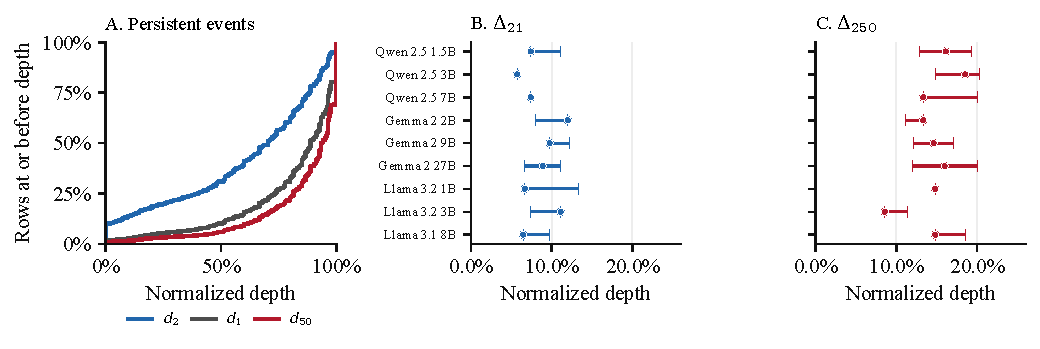
\includegraphics[width=\linewidth]{figure1_staged_summary.pdf}
\caption{\textbf{Answer formation is staged across depth.} Left: persistent contender status, persistent winner status, and persistent decisive margin arrive at different depths. Middle/right: model-level median lags with 95\% bootstrap intervals.}
\label{fig:staged-summary}
\end{figure*}

The separation among the three curves means that contender status, winner status, and decisive separation are not interchangeable readouts. A row can already carry the eventual answer among the leading options while the final-pair margin is still being written. Endpoint accuracy and final margins collapse these events into one terminal observation.

The main lag is $\Delta_{250}$, from persistent contender status to persistent decisive margin. Its pooled median is \PooledMedianDeltaTwentyFifty{}, with a 95\% bootstrap interval of [\PooledDeltaTwentyFiftyLow{}, \PooledDeltaTwentyFiftyHigh{}]. The smaller lag $\Delta_{21}$, from persistent contender to persistent top-1, has pooled median \PooledMedianDeltaTwentyOne{} with interval [\PooledDeltaTwentyOneLow{}, \PooledDeltaTwentyOneHigh{}].

Across models, the lags in Figure~\ref{fig:staged-summary} occupy a visible part of model depth rather than a single boundary layer. This staged view is the organizing principle for the rest of the paper. Candidate formation, winner selection, and decisive separation are related but distinct events in the score trajectory.

\section{Final separation is often written late}

Once the final answer has become a persistent contender, the trajectory is not finished. The final-pair gap can still be small, and later layers often add much of the eventual separation. We measure this by summing positive increases in the final winner-versus-runner-up gap and asking how much of that positive write occurs after key events.

\begin{figure}[tbp]
\centering
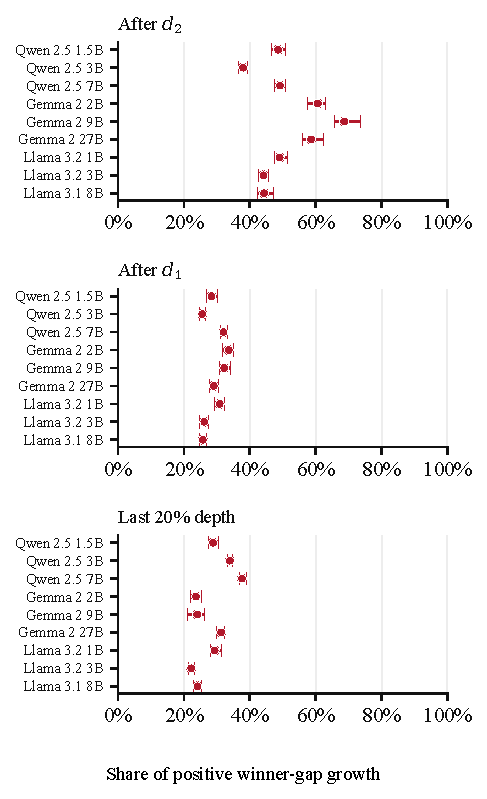
\includegraphics[width=\linewidth]{figure3_late_write.pdf}
\caption{\textbf{Much of the final winner-gap growth occurs after contender status.} Each point is a model median; intervals are 95\% bootstrap intervals. The broad panel shows that contender formation does not imply immediate isolation.}
\label{fig:late-write}
\end{figure}

The pooled median share of positive winner-gap growth written after $d_2$ is \PooledWriteAfterDTwo{}. Even after persistent top-1 status, the median remaining positive write is \PooledWriteAfterDOne{}. This makes late write a natural companion to the persistence-depth result: the model can have selected the eventual answer while still continuing to strengthen it.

This is why late write is not redundant with persistent winner status. Persistent top-1 says that the final answer has stopped losing to another option; late write says that the gap separating it from the runner-up is still being actively increased.

This is a readout-space statement. It does not by itself identify which internal components create the late write. The instrumented panel below asks that narrower mechanistic accounting question.

\section{Trajectories form regimes}

The staged quantities also support a compact regime view. We label broad-panel rows by whether they are stable-correct, stable-wrong, late-crystallizing, switch-heavy, or unstable under deterministic criteria from the cached trajectory. These labels are descriptive: they organize how the answer forms, rather than asserting a discontinuous phase transition.

\begin{figure}[tbp]
\centering
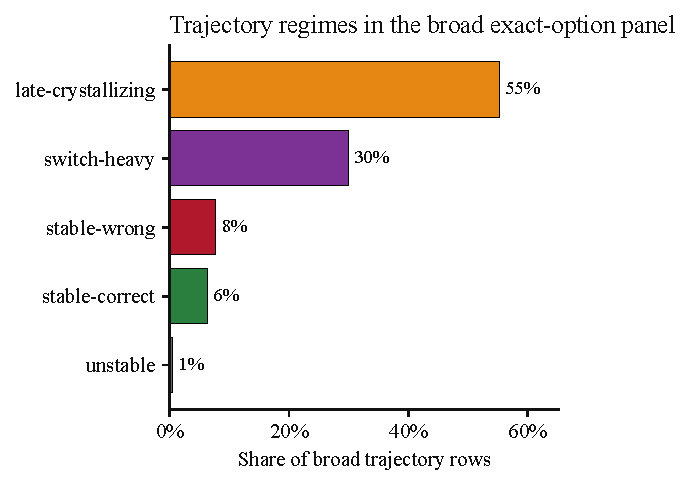
\includegraphics[width=0.96\linewidth]{figure4_regime_summary.pdf}
\vspace{0.25em}
{\small\begin{tabular}{@{}lrr@{}}
\toprule
\textbf{Trajectory regime} & \textbf{Rows} & \textbf{Share} \\
\midrule
late-crystallizing & 4924 & 55\% \\
switch-heavy & 2672 & 30\% \\
stable-wrong & 688 & 8\% \\
stable-correct & 572 & 6\% \\
unstable & 45 & 1\% \\
\bottomrule
\end{tabular}
}
\caption{\textbf{Answer-formation regimes in the broad panel.} Bars show regime shares; the table reports the exact released counts. Late-crystallizing and switch-heavy trajectories are common, showing why endpoint accuracy alone is a thin summary of answer formation.}
\label{fig:regimes}
\end{figure}

The regime view connects the staged result to heterogeneity. Some rows become stable early, some carry the correct answer late, and some continue switching leaders deep into the network. The same persistence and switch-count quantities produce all regimes, so the labels summarize trajectory shape without introducing a separate measurement target.

Across models, median $\Delta_{250}$ ranges from \MinMedianDeltaTwoFifty{} to \MaxMedianDeltaTwoFifty{}, and median write after $d_2$ ranges from \MinWriteAfterDTwo{} to \MaxWriteAfterDTwo{}. The qualitative ordering of candidate formation before winner isolation remains the common structure.

\section{Mechanistic accounting of margin drift}

The broad panel shows staged answer formation. The instrumented panel asks what can be said about the motion itself. For each layer, the cache contains margin drift along with attention and MLP scalar contributions. A linear drift decomposition reaches held-out $R^2$ between \MechanisticMinHeldoutRtwo{} and \MechanisticMaxHeldoutRtwo{} across the three instrumented models, which is strong enough to treat the decomposition as useful accounting of readout motion.

\begin{figure}[tbp]
\centering
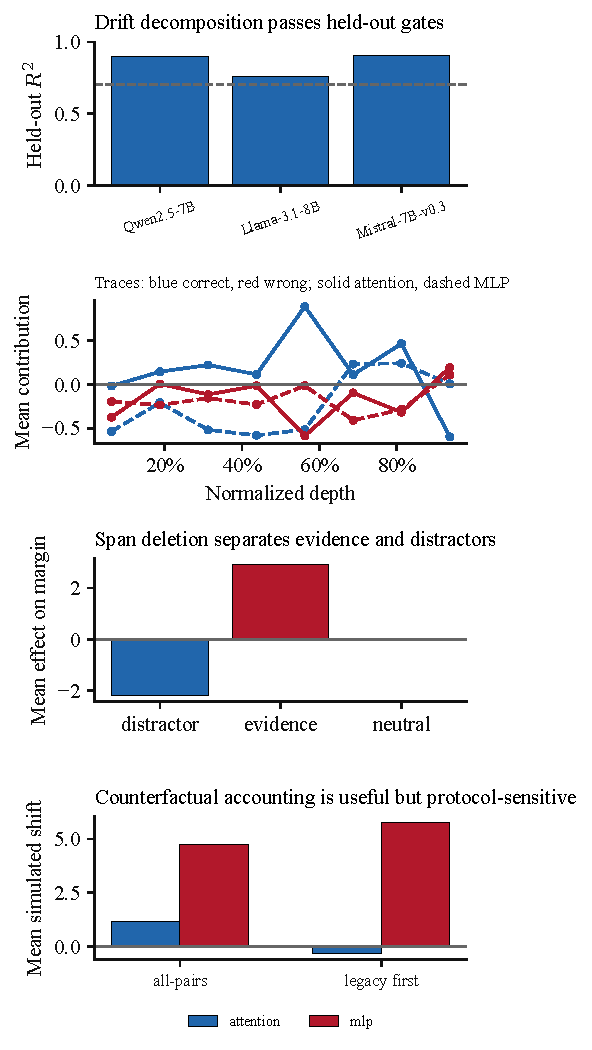
\includegraphics[width=\linewidth]{figure5_mechanistic_accounting.pdf}
\caption{\textbf{Mechanistic accounting in the instrumented panel.} Attention/MLP scalars reconstruct margin drift with held-out fits; component traces differ by trajectory type; span deletion separates evidence from distractors; and substitution accounting is informative but protocol-sensitive.}
\label{fig:mechanistic}
\end{figure}

The panels in Figure~\ref{fig:mechanistic} play different roles. The held-out fits show that a low-dimensional accounting model captures margin drift; the trace panel shows that component contributions vary by trajectory type; span deletion is the strongest input-level intervention; and substitution is useful but more protocol-sensitive.

The strongest intervention evidence is span deletion. Evidence spans have positive mean effects on the decision margin, while distractor spans have negative mean effects; the mean evidence-minus-distractor gap is \SpanEvidenceDistractorGap{} logit-margin units. The effect remains significant under Benjamini--Hochberg correction, and observed effects exceed shuffled and sign-flipped controls.

\begin{table}[tbp]
\centering
\small
\begin{tabularx}{\linewidth}{@{}lX@{}}
\toprule
\textbf{Mechanistic artifact} & \textbf{Value} \\
\midrule
Instrumented models & 3 \\
Component-depth summary rows & 288 \\
Minimum held-out drift R-squared & 0.76 \\
Mean evidence-minus-distractor gap & 5.10 \\
All-pairs MLP substitution mean shift & 4.74 \\
All-pairs attention substitution mean shift & 1.18 \\
\bottomrule
\end{tabularx}

\caption{\textbf{Mechanistic artifact summary.} All values are regenerated from the released mechanistic table.}
\label{tab:mechanistic-summary}
\end{table}

Cached counterfactual accounting adds a second, more conditional result. Under order-invariant all-pairs substitution, attention shifts failing trajectories by \SubstitutionAttentionMean{} logits on average, while MLP shifts them by \SubstitutionMLPMean{} logits on average. This supports the qualitative conclusion that MLP contributions are often more transferable in the cached accounting setup. It is not an unconditional circuit claim: the exact sign and magnitude vary with pairing protocol, layer range, and normalization.

\section{Sensitivity and limits}

The broad result depends on exact-option continuation scoring under canonical answer ordering. That is the intended primary readout because it scores the answer string itself rather than a proxy label. Alternate readouts and option orders are useful sensitivity material, but they can change the final winner and therefore are not used to replace the primary path.

Several edge cases are handled explicitly. Final-layer ties are logged, and rows with nonpositive final gaps are excluded from normalized-gap metrics rather than forced into $d_{50}$. Across included broad-panel rows, \FinalLayerTieCount{} rows have a final-layer top tie and \NormalizedGapExcludedCount{} rows are excluded from normalized-gap metrics. The appendix reports neighboring thresholds, $25\%$ and $75\%$, to show how the margin-depth timing shifts when the criterion is relaxed or tightened.

The mechanistic results also have a boundary. The attention/MLP decomposition is a scalar accounting model over cached readouts. Span deletion is a true input-level intervention in the legacy cache. Simulated ablation and substitution are linearized bookkeeping estimates: they do not let later layers react to a modified activation state. We therefore use them to support conditional component-level patterns, not to claim complete causal circuits.

The empirical scope is multiple-choice cached readouts in the tested open-weight models and benchmarks. The paper does not claim behavior for open-ended generation, all architectures, or all answer formats.

\section{Conclusion}

Endpoint accuracy hides the shape of answer formation. In cached multiple-choice readouts, the final answer usually becomes a contender before it becomes the winner, and it often continues to gain separation late in depth. Regime labels make this variation visible: stable, late-crystallizing, switch-heavy, and unstable trajectories are different ways for the same endpoint interface to arise.

The instrumented panel shows that this is not only a descriptive curiosity. Attention/MLP scalars provide useful accounting of margin drift, and span deletion with controls shows that evidence and distractor spans move the margin in opposite directions. The result is a coherent, reproducible map of answer formation: broad enough to show the phenomenon across models, and instrumented enough to begin explaining where the motion comes from.


\bibliographystyle{plainnat}
\bibliography{references}

\appendix
\balance
\section{Reproducibility and release QA}

The release rebuilds from included derived data and does not require model weights, GPU access, Hugging Face access, or new inference. The rebuild entry point is \texttt{scripts/rebuild\_all.py}. It regenerates paper-facing tables, figures, LaTeX macros, the PDF, rendered page PNGs, and hash manifests. The optional raw-cache verification path is described in \texttt{REPRODUCE.md}.

\subsection{Dataset counts}

\begin{center}
\small
\begin{tabular}{@{}lrr@{}}
\toprule
\textbf{Dataset} & \textbf{Prompts} & \textbf{Role} \\
\midrule
ARC-Challenge & 195 & broad trajectory panel \\
CommonsenseQA & 794 & broad trajectory panel \\
\bottomrule
\end{tabular}

\captionof{table}{\textbf{Dataset counts included in the release.} The broad trajectory panel uses ARC-Challenge and CommonsenseQA.}
\label{tab:dataset-counts}
\end{center}

\subsection{Threshold sensitivity}

\begin{center}
\small
\begin{tabular}{@{}lrrr@{}}
\toprule
\textbf{Metric} & \textbf{Valid} & \textbf{Median} & \textbf{95\% CI} \\
\midrule
$d_{25}$ & 8856 & 0.93 & [0.91, 0.93] \\
$d_{50}$ & 8856 & 0.94 & [0.93, 0.94] \\
$d_{75}$ & 8856 & 0.96 & [0.96, 0.97] \\
$\Delta_{21}$ & 8901 & 0.09 & [0.08, 0.10] \\
$\Delta_{250}$ & 8856 & 0.15 & [0.13, 0.15] \\
\bottomrule
\end{tabular}

\captionof{table}{\textbf{Pooled threshold and lag summary.} Values are normalized-depth medians with 95\% bootstrap intervals.}
\label{tab:threshold-summary}
\end{center}

\subsection{QC summary}

The generated QC table is included in the release artifacts. It records \FinalLayerTieCount{} final-layer top ties and \NormalizedGapExcludedCount{} rows excluded from normalized-gap metrics; missing option scores, missing options by layer, final-winner mismatches, and nonmonotonic layer-index rows are all zero.


\end{document}
